\hypertarget{ux4e0aux4e0bux6587ux4e0eux8bb0ux5fc6}{%
\chapter{上下文与记忆}\label{ux4e0aux4e0bux6587ux4e0eux8bb0ux5fc6}}

\hypertarget{ux68c0ux7d22ux589eux5f3aux751fux6210}{%
\section{检索增强生成}\label{ux68c0ux7d22ux589eux5f3aux751fux6210}}

\hypertarget{ux4e00ux68c0ux7d22ux589eux5f3aux751fux6210ragux7684ux57faux672cux65b9ux6cd5}{%
\subsection{一、检索增强生成（RAG）的基本方法}\label{ux4e00ux68c0ux7d22ux589eux5f3aux751fux6210ragux7684ux57faux672cux65b9ux6cd5}}

LLM尽管通用能力较强，但知识范围、实时性以及回答时知识定位的精确度都仍然有限。为此我们让模型在回答问题时实时检索，为回答提供参考。

（一）RAG的标准流程

首先构建知识库，即对自然语言文本等非结构化数据的向量化存储。为了保存语义信息并方便后续的相似度检索，我们将文本裁切为片段，并训练一个嵌入模型，将这些片段分别转换为嵌入向量（embedding vector）并建立索引。

在生成时，我们会用Query（查询）向量在知识库中相似度检索，找到最相关的内容加入上下文（或将其所在的整篇文献加入上下文）。对于文本知识库，我们往往用余弦相似度，因为它更关注语义方向的相似性，而不受文本长度等无关因素的影响。而有时为了避免漏掉精确关键词，往往会和BM25等传统关键字检索方法结合，如finalScore = (0.7 * vectorScore) + (0.3 * textScore)。

原始的RAG采取``先检索后生成''，即顺序架构：Query → Retrieve → Generate。

（二）动态决定调用搜索工具

我们可以在模型的词表中加入\texttt{\textless{}search\textgreater{}} token，生成后即调用搜索API。可以通过在训练数据中加入调用示例，或者通过强化学习的方式让模型在自主探索中学会在需要搜索时生成\texttt{\textless{}search\textgreater{}} token，调用检索辅助完成任务。

\begin{enumerate}
\def\labelenumi{\arabic{enumi}.}
\tightlist
\item
  架构分类
\end{enumerate}

（1）条件架构：可以引入``判断器 (Judger/Router)''，根据问题的难度或类型决定是否检索，或如何检索，也可以通过强化学习的方式让模型自主学会判断是否搜索（即是否生成\texttt{\textless{}search\textgreater{}} token）。

（2）分支架构：并行执行多条路径，通过集成或排序来融合结果。

概率集成：将每个检索到的文档分别输入LLM计算生成概率，最后将多个文档对应的生成概率分布进行加权融合。

候选排序：让LLM基于每个文档分别生成答案，然后根据生成的置信度或相关性对这些答案进行排序，选择最好的一个。

（3）循环/迭代架构：检索和生成交替进行，形成闭环，Retrieve → Generate，适用于长文本生成或复杂多步推理。

交替迭代：生成一部分 → 拿着生成的内容去检索新信息 → 基于新信息继续生成 → 循环。

主动触发：在生成过程中监测生成概率。如果 LLM 对当前生成的词``犹豫不决''（概率低），则立即触发检索，用检索到的信息``纠正''生成方向。

反思与自纠：训练LLM输出特殊的反思Token，判定是否需要检索，检索到的内容是否相关，生成的内容是否有用。

\begin{enumerate}
\def\labelenumi{\arabic{enumi}.}
\setcounter{enumi}{1}
\tightlist
\item
  训练方法
\end{enumerate}

（1）监督微调：需要高质量标注轨迹，且搜索操作本身的不可微性使得端到端优化变得困难。

（2）结合检索的强化学习：仅通过最终结果的奖励（Outcome-based Reward），让模型自主学会``思考-检索-再思考-回答''的交替流程，用PPO、GRPO等强化学习算法。

需要注意的是，在计算策略梯度时，轨迹y中既包含模型生成的 Token，也包含搜索引擎返回的固定Token。如果不加区分地训练，模型可能会试图``优化''检索到的文本，或者被检索内容的分布带偏。``检索''只是一个动作，模型通过强化学习（RL）的奖励机制学会的是何时输出\texttt{\textless{}search\textgreater{}}标记。故我们运用掩码机制，把搜索到的文本Token（不包含\texttt{\textless{}search\textgreater{}} token）加上掩码，只以其他token作为RL优化的策略。

（三）自适应RAG

在标准RAG中，在引入需要的信息的同时往往也引入了大量无关信息。为避免上下文无关信息的积累，可将检索到的信息分割成较小的块，每次输入一个块，并调用LLM回答，如此循环，直至得到需要的答案停止。由于KV Cache的存在，时间复杂度仍然是线性增长的（也就是和标准RAG一致），只要需要的信息不是在最后一个块里，理论上就能起到加速作用。

较大的块成功召回需要的信息的概率更大，但同时也会引入更多无关信息（干扰项）；较小的窗口虽能减少干扰，但要求模型在更多块中准确拒绝无关信息块，增加错误拒绝需要的信息块以及累计错误的风险。

（四）稀疏检索与稠密检索

稀疏检索即传统关键词检索方法，如BM25。稠密检索即利用Embedding向量检索的方法。相较于稀疏检索而言，稠密检索能更好地利用语义层面的信息。

实践中常采取稠密和稀疏索引结合的方法。如Claude-mem：查询先走Chroma向量检索（基于语义相似度的稠密检索），召回Top 100结果，再做90天时间窗口过滤，最后用SQLite（稀疏检索）按时间顺序补全/重排数据。

\hypertarget{ux4e8cux7a20ux5bc6ux68c0ux7d22}{%
\subsection{二、稠密检索}\label{ux4e8cux7a20ux5bc6ux68c0ux7d22}}

（一）嵌入向量的选取

\begin{enumerate}
\def\labelenumi{\arabic{enumi}.}
\tightlist
\item
  切成片段（Chunk）
\end{enumerate}

一般而言，一个嵌入向量会取256-1024 tokens，或者一个自然段，以包含一个完整的论点或逻辑段落。还可以计算相邻句子的相似度，如果相似度突降，说明话题变了，就在这里切。

为什么要这么做？如果把每一个词或每一句话单独做成向量，虽然粒度很细，但会因为缺乏上下文而导致语义偏离，检索时容易出错。如一个知识库把一个句子作为一个嵌入向量，有一个句子是``它崩溃了''。将其单独变为embedding向量，向量化后包含了``崩溃''的语义，但缺乏上下文，丢失了主语（是服务器崩溃，还是股市崩溃？）。检索时，在服务器、股市等很多场景检索时，这句话都会被检索到。也就是说，检索时会召回大量无关内容。而如果把整篇5000字的论文做成一个向量，要么需要很高的embedding维度（计算复杂度增大），要么在不改变维度的情况下把文章里不同内容的语义混合在向量里（向量的方向会变得模糊）。所谓``文档向量''，一般实际上就指的是片段对应的向量。

另外，我们不会硬生生切断，通常会设置10\%\textasciitilde20\%的重叠（例如50 Tokens），防止某个关键句子刚好被切在两块的连接处，导致语义断裂。

\begin{enumerate}
\def\labelenumi{\arabic{enumi}.}
\setcounter{enumi}{1}
\tightlist
\item
  切片的改进
\end{enumerate}

虽然切片是主流，但切片可能失去了上下文（例如，一个切片里写着``这个方案能将准确率提高20％''，但切片里没有写``这个方案''是什么）。对此有两种改进方法：（1）搜索到片段后，把其所在全文都输入给LLM；（2）在片段embedding时，将全文压缩后的摘要作为上下文输入供参考。

（二）嵌入向量的存储介质

一般而言，被检索的嵌入向量保存在CPU内存中（或量化压缩后保存在CPU内存中）。如果数据量过大，可将索引向量压缩在内存，指向的原始文本数据存在SSD中。

由于嵌入向量在CPU内存中，在数据量不大的情况下，在推理时直接运用CPU计算可避免I/O阻塞耗时。如果数据量大、高并发必须使用GPU，则应将量化压缩后的索引向量集存入GPU显存，再取如Top-1000从CPU中取入GPU精确计算。

（三）嵌入模型的训练

由于``选取最相关的一些文本加入上下文''运用了不可导的Top-K操作，嵌入模型无法直接和主LLM一起端到端训练，而需要另行训练。

\begin{enumerate}
\def\labelenumi{\arabic{enumi}.}
\tightlist
\item
  对比学习
\end{enumerate}

用语义相似的文本为正样本（如论文和它的摘要、论坛的问题和回答、新闻的标题和正文等），语义不同的为负样本（批次内非正样本均可视为负样本，此外还可以找辨析难度更大的困难样本，如讲水果中的苹果和苹果手机的段落）。

假设我们有一个查询 \(q\)（Query）和一个相关的文档 \(d^+\)（Positive Document），以及 \(N\) 个不相关的文档 \(d^-\)（Negative Documents）。

我们使用 InfoNCE Loss（Information Noise Contrastive Estimation）作为损失函数。这是目前训练 Embedding 最主流的公式：

\[
\mathcal{L}=-\log\frac{\exp(\mathrm{sim}(q,d^+)/\tau)}{\sum_{i=0}^{N}\exp(\mathrm{sim}(q,d_i)/\tau)}
\]

其中：

\begin{itemize}
\tightlist
\item
  \(\mathrm{sim}(u,v)\) 是两个向量的余弦相似度：\(\mathrm{sim}(u,v)=\frac{u^\top v}{\lVert u\rVert\lVert v\rVert}\)。
\item
  \(d^+\) 是正样本。
\item
  \(d_i\) 包含 1 个正样本和 \(N\) 个负样本。
\item
  \(\tau\) 是温度系数（Temperature），用于控制模型对困难样本的敏感度。
\end{itemize}

\begin{enumerate}
\def\labelenumi{\arabic{enumi}.}
\setcounter{enumi}{1}
\tightlist
\item
  蒸馏生成模型的注意力分布
\end{enumerate}

字面相似度往往具有欺骗性，嵌入向量``是否相似''应当取决于内容逻辑，这是在复杂的生成过程中体现的。如：Query：``治疗阿尔茨海默病的新靶点。''文档A（字面相似）：一篇综述，标题包含``阿尔茨海默病治疗''，但内容全是老旧信息。文档B（字面不相似）：讨论``蛋白折叠异常与神经元坏死''，没提``阿尔茨海默''这个词，但内容逻辑正是通过解决蛋白折叠来治疗该病。

我们希望用下游任务的效用来监督上游检索的排序。尽管我们无法端到端优化嵌入模型，但可以让它生成的概率模仿生成器的Attention中各个token出现的概率，也就是运用蒸馏的方法：

第一步：获取生成器的``注意力分布'' \(P_{\mathrm{Teacher}}\)。

假设检索回了 \(K\) 个文档 \(\{D_1,D_2,\ldots,D_K\}\)。当生成器生成答案 \(Y\) 时，我们可以查看 Cross-Attention（或者 Decoder-Only 模型的 Self-Attention）层中的权重。

我们将生成器对第 \(i\) 个文档的所有 token 的注意力权重进行聚合（例如求和或取平均），得到该文档的重要性分数 \(A_i\)。然后进行归一化：

\[
P_{\mathrm{Gen}}(D_i\mid Q)=\frac{\exp(A_i/\tau)}{\sum_{j=1}^{K}\exp(A_j/\tau)}
\]

这个 \(P_{\mathrm{Gen}}\) 就是真理：它代表了``在生成答案时，第 \(i\) 篇文档实际上贡献了多少''。

第二步：获取检索器的``检索概率'' \(P_{\mathrm{Student}}\)。

检索器（通常是双塔模型）计算 Query 和 Document 的点积分数 \(S_i=E_Q\cdot E_{D_i}\)。我们也对它进行 Softmax 归一化：

\[
P_{\mathrm{Ret}}(D_i\mid Q)=\frac{\exp(S_i)}{\sum_{j=1}^{K}\exp(S_j)}
\]

第三步：计算损失并蒸馏（Distillation）。

我们要让检索器的分布 \(P_{\mathrm{Ret}}\) 尽可能接近生成器的分布 \(P_{\mathrm{Gen}}\)。通常使用 KL 散度（Kullback-Leibler Divergence）作为损失函数：

\[
\mathrm{Loss}=\mathrm{KL}(P_{\mathrm{Gen}}\Vert P_{\mathrm{Ret}})=\sum_i P_{\mathrm{Gen}}(D_i\mid Q)\log\frac{P_{\mathrm{Gen}}(D_i\mid Q)}{P_{\mathrm{Ret}}(D_i\mid Q)}
\]

关键点：这个 Loss 是可导的，可以通过梯度下降更新检索器的参数（即更新 Query Encoder 的权重），让检索器学会：``原来在这个问题下，虽然文档 B 只有 \(0.6\) 的相似度，但它应该排第一。''

\hypertarget{ux4e09ux91cdux6392ux5e8fux4e0eux7cbeux70bc}{%
\subsection{三、重排序与精炼}\label{ux4e09ux91cdux6392ux5e8fux4e0eux7cbeux70bc}}

（一）重排序器

\begin{enumerate}
\def\labelenumi{\arabic{enumi}.}
\tightlist
\item
  全量重排序
\end{enumerate}

前面的稀疏和稠密检索可以让我们获得Top-K分数的文档（片段），但都主要集中在整个文档（片段）向量的整体语义上，为了速度牺牲了精度。为此，我们还需要进一步在token级别进行精细化调整，即用重排序器，在检索出的 Top-K（例如前100个）文档上进行排序。具体方法有：

（1）LLM评估法

（2）交叉编码器法

输入构造：将查询 \(q\) 和候选文档 \(d\) 拼接成一个序列，中间用分隔符隔开：

\[
\mathrm{Input}=[\mathrm{CLS}]\oplus q\oplus[\mathrm{SEP}]\oplus d\oplus[\mathrm{SEP}]
\]

全注意力交互（Full Self-Attention）：将拼接后的序列输入 Transformer。由于 Self-Attention 机制，查询中的每个 token 都能注意到文档中的每个 token。这使得模型能理解复杂的逻辑关系（如否定词``不''、``但是''）。

评分输出：通常取 \([\mathrm{CLS}]\) 标记的输出向量，经过一个全连接层（Linear Layer），输出一个标量分数 \(s\in[0,1]\)（通常经过 Sigmoid）。

\[
\mathrm{Score}(q,d)=\sigma\left(W\cdot\mathrm{Transformer}(\mathrm{Input})_{[\mathrm{CLS}]}+b\right)
\]

可以看到，这里并非Query对文档用互注意力（Bi-Encoder），而是Query和文档拼接后用自注意力打分（Cross-Encoder）。最后取Query {[}CLK{]}对应的全局注意力向量，追求极致的精度。（注：W为1*d\_model维，和{[}CLS{]}token向量的d\_model*1维相乘为标量）

为什么选择交叉编码器：

\begin{itemize}
\tightlist
\item
  \textbf{双编码器（Bi-Encoder）}：

  \begin{itemize}
  \tightlist
  \item
    流程：Query \(\to\) Vector \(V_q\)，Doc \(\to\) Vector \(V_d\)。
  \item
    计算：\(V_q\cdot V_d\)。
  \item
    痛点：Query 和 Doc 在生成向量时是互不可见的。所有的语义必须被压缩到一个固定维度的向量中（Vector Bottleneck）。例如，``苹果''这个词，在生成向量时必须同时隐含``水果''和``公司''的含义，非常模糊。
  \end{itemize}
\end{itemize}

``互不可见''指的就是：在生成 \(V_d\) 的那一刻，模型不知道 \(Q\) 是什么；在生成 \(V_q\) 的时刻，模型不知道 \(D\) 是什么。它们是独立编码的。假设有一篇文档 \(D\)：``苹果发布了新财报，股价大涨。''

\begin{itemize}
\tightlist
\item
  \textbf{场景 A（Cross-Encoder，无瓶颈）}：

  \begin{itemize}
  \tightlist
  \item
    Query：``好吃的水果有哪些？'' \(\to\) 拼接后模型看到``水果''和``股价''，直接打低分。
  \item
    Query：``科技公司动态'' \(\to\) 拼接后模型看到``科技''和``股价''，打高分。
  \item
    模型在交互中动态理解了语义。
  \end{itemize}
\item
  \textbf{场景 B（Bi-Encoder，有瓶颈）}：

  \begin{itemize}
  \tightlist
  \item
    文档 \(D\) 必须被压缩成一个静态向量 \(V_d\)。
  \item
    这个 \(V_d\) 必须同时通过 768 个数字来表达``苹果''``公司''``赚钱''``科技''等所有含义。- \textbf{多义词灾难}：
  \item
    如果 \(V_d\) 过分强调``科技''，那遇到 Query ``苹果（水果）''时，虽然语义不符，但因为都含有``Apple''这个词的嵌入信息，向量距离可能还是很近（产生幻觉/误召回）。
  \item
    如果 \(V_d\) 试图中庸，既像水果又像科技，那它可能离``纯粹的水果''和``纯粹的科技''都有一段距离，导致谁都搜不到它。
  \end{itemize}
\end{itemize}

总结：Vector Bottleneck 指的是：无论句子多长、含义多丰富、多歧义，双编码器都强行将其压缩进一个固定大小的向量中。由于缺乏查询时的上下文（Context），这个向量只能是一个``模糊的平均值''，丢失了细粒度的语义匹配能力。

而如果用交叉编码器，模型在Embedding时可直接将Query和文档拼接，根据Query确定把文档的哪些内容放进Embedding。但缺点是这样文档的Embedding依赖于Embedding，必须在每次给出Query后都在线计算，而无法提前单独对文档进行Embedding操作。

\begin{enumerate}
\def\labelenumi{\arabic{enumi}.}
\setcounter{enumi}{1}
\tightlist
\item
  chunk重排序
\end{enumerate}

在数据量大、对延时要求高、算力相对不足等情形下，对所有的论文进行整个文档的token级计算并不现实，往往每篇论文只能取几个较小的chunk送进重排序器（如果是论文检索等场景，往往除了chunk之外还会加上摘要一并送入重排序器）。一般而言，切分chunk的方法有：

（1）按自然段/一定token数切分：每段或每一定token数为一个chunk，最简便，但有时会丢失一些上下文信息，或出现冗余信息。可以通过加入压缩后的上下文、与相邻chunk 20\%重叠的方式一定程度上解决丢失上下文信息的问题，保证连续性。

（2）按句子切分再合并：先按句子切分，再计算每一句与下一句的embedding向量间的相似度。若高于阈值，则将下一句合并入该句所在chunk；否则二者分入不同chunk。这样可以得到若干chunk。

切分完毕后，计算Query与每个小chunk的embedding向量间的相似度，取每篇论文TopK的chunk，送进重排序器。

（二）精炼器

检索到的文档往往包含大量无关噪声，直接输入生成器会导致Token浪费甚至产生幻觉。精炼器的目标是提高``信噪比''，故常用精炼器进行精炼后再加入上下文窗口。精炼方法：

\begin{enumerate}
\def\labelenumi{\arabic{enumi}.}
\item
  抽取式精炼：使用一个轻量级的打分模型（甚至可以是另一个 Cross-Encoder）对每个句子评分，判断其是否包含回答问题所需的关键信息。
\item
  摘要式精炼：让LLM或小型BERT模型对检索到的内容生成摘要。
\item
  LLMLingua压缩：用LLM预测对应token，越能被轻易预测，该token信息量（困惑度）越小，越应压缩。
\end{enumerate}

\[
\mathrm{Keep}(x_t)=\mathbf{1}\!\left[-\log P\!\left(x_t\mid x_{<t}\right)>\tau\right]
\]

\hypertarget{ux53c2ux8003ux6587ux732e-124}{%
\subsection{参考文献}\label{ux53c2ux8003ux6587ux732e-124}}

\vspace{0.25em}
\begin{itemize}
\tightlist
\item
  《动手学大模型智能体》。
\item
  Jin, B., Zeng, H., Yue, Z., et al.~(2025). \href{https://arxiv.org/abs/2503.09516}{Search-R1: Training LLMs to Reason and Leverage Search Engines with Reinforcement Learning}. arXiv:2503.09516.
\item
  Robertson, S., \& Zaragoza, H. (2009). \href{https://doi.org/10.1561/1500000019}{The Probabilistic Relevance Framework: BM25 and Beyond}. Foundations and Trends in Information Retrieval, 3(4), 333-389.
\item
  Manning, C. D., Raghavan, P., \& Schütze, H. (2008). \href{https://nlp.stanford.edu/IR-book/}{Introduction to Information Retrieval: Okapi BM25, a non-binary model}. Cambridge University Press.
\item
  thedotmack. (2026). \href{https://github.com/thedotmack/claude-mem}{claude-mem GitHub repository}.
\item
  van den Oord, A., Li, Y., \& Vinyals, O. (2018). \href{https://arxiv.org/abs/1807.03748}{Representation Learning with Contrastive Predictive Coding}. arXiv:1807.03748.
\item
  Izacard, G., \& Grave, E. (2021). \href{https://arxiv.org/abs/2012.04584}{Distilling Knowledge from Reader to Retriever for Question Answering}. ICLR 2021.
\item
  Nogueira, R., \& Cho, K. (2019). \href{https://arxiv.org/abs/1901.04085}{Passage Re-ranking with BERT}. arXiv:1901.04085.
\item
  Reimers, N., \& Gurevych, I. (2019). \href{https://arxiv.org/abs/1908.10084}{Sentence-BERT: Sentence Embeddings using Siamese BERT-Networks}. EMNLP 2019.
\item
  Xu, F., Shi, W., \& Choi, E. (2023). \href{https://arxiv.org/abs/2310.04408}{RECOMP: Improving Retrieval-Augmented LMs with Compression and Selective Augmentation}. ICLR 2024.
\item
  Jiang, H., Wu, Q., Lin, C.-Y., Yang, Y., \& Qiu, L. (2023). \href{https://arxiv.org/abs/2310.05736}{LLMLingua: Compressing Prompts for Accelerated Inference of Large Language Models}. EMNLP 2023.
\end{itemize}

\clearpage

\hypertarget{ux6a21ux578bux7684ux8bb0ux5fc6}{%
\section{模型的记忆}\label{ux6a21ux578bux7684ux8bb0ux5fc6}}

\hypertarget{ux4e00ux77edux671fux8bb0ux5fc6ux4e0aux4e0bux6587}{%
\subsection{一、短期记忆（上下文）}\label{ux4e00ux77edux671fux8bb0ux5fc6ux4e0aux4e0bux6587}}

短期记忆是大模型执行任务时对当前任务上下文的记忆，对应``上下文学习''，其底层实现是注意力中存储的KV Cache，任务结束后即清空。

由于硬件显存有限，大模型的上下文窗口长度有限，如果超出长度就必须采取一些机制。对于短期记忆自身而言，可以采取的措施例如：

\begin{enumerate}
\def\labelenumi{\arabic{enumi}.}
\item
  滑动窗口：保留最近的K轮对话。
\item
  摘要：对于更早的内容，生成摘要，并``遗忘''原内容，一般和滑动窗口配合使用。摘要会暂时储存在内存中，并加入后续对话的上下文窗口。
\end{enumerate}

后续还会有和长期记忆配合的一些其他方法。

\hypertarget{ux4e8cux957fux671fux8bb0ux5fc6}{%
\subsection{二、长期记忆}\label{ux4e8cux957fux671fux8bb0ux5fc6}}

我们可以通过向量数据库的形式，将记忆内容嵌入为语义向量，保存在大容量介质（如硬盘）中。例如，OpenClaw将记忆存储在工作区的特定markdown文件中。在运用时，根据请求用向量相似度在数据库中检索，获取最相关的内容，也可以通过提示词让模型以其他方式灵活调取。记忆内容可以包括历史问答及其摘要、垂直领域知识、执行动作的历史及经验教训、用户偏好等。

在上下文超过短期记忆上限时，我们可以将最早的历史信息（或只存其摘要）移动到长期记忆中，在后续如果被检索到（即需要这些信息）则再加入短期记忆。

由于长期记忆读写速度慢，我们一般不会每次对话都访问，而是在初始化（开始工作前）、检索（遇到一定的问题或场景，LLM判断需要调用记忆）或归档（项目做完打包结项）等时候按需要调用。

长期记忆可以分层，如OpenClaw包括一个大数据库和一个精选过的最重要的记忆（如用户偏好、重要决定等），每次涉及与用户对话时都会调取精选记忆。以Claude-mem为例，其采取了``渐进式披露''的方法，在通过检索方法（稠密检索、稀疏检索）得到若干条记忆条目后，不立即全部注入上下文，而是分层处理。具体而言，就是在建立记忆时，就分为如下三层，从而在调用时分层读取：

Layer 1：Search（索引层）：一个``轻量索引''，每一行包括该条记忆的ID、时间、类别、标题、token成本，例如：\textbar{} \#2102\textbar{} Oct 20 \textbar{} problem-solution \textbar{} Fixed timeout in CI \textbar{} 100 tokens \textbar。如gotcha表示这是个坑，problem-solution表示这是曾经的问题与解法等。对于检索到的条目，将它们的索引层注入主模型，模型看标题和类型就能判断：这一条是否有必要调用更贵的Layer 2 / Layer 3。（这里和前面的检索的不同点在于，检索是运用固定的检索算法，因而比较粗略，无法处理精细语义；这里虽然只有少量浓缩信息，但模型可以根据需要灵活判断）

Layer 2：Timeline（时间线层）：事件记忆，类似于日志。当模型在Layer 1中选定ID后，对于每个ID，拉出它的前后几条时间线，看看这步操作的前后都发生了什么。

Layer 3：Get Observations（详情层）：对Layer 1中选定的ID，如果经过读取Layer 2后，模型仍认为需要更多信息，则会拉取该ID对应的完整结构化内容。例如：

\#2543 Hook timeout: 60s too short for npm install

─────────────────────────────────────────────────

Date: Oct 26, 2025 2:14 PM

Type: gotcha

Project: claude-mem

Narrative:

Discovered that the default 60-second hook timeout is insufficient

for npm install operations, especially with large dependency trees

or slow network conditions. This causes SessionStart hook to fail

silently, preventing context injection.

Facts:

- Default timeout: 60 seconds

- npm install with cold cache: \textasciitilde90 seconds

- Configured timeout: 120 seconds in plugin/hooks/hooks.json:25

Files Modified:

- plugin/hooks/hooks.json

Concepts: hooks, timeout, npm, configuration

总而言之，这里的结构化信息包括：

Narrative（叙事）：

用自然语言描述``发生了什么、问题是什么、影响是什么''，方便 Agent 理解上下文。

Facts（事实清单）：

关键数值、配置项、结论，方便做逻辑推理。

Files Modified / Files Read：

直接告诉 Agent：这个观察跟哪些文件有关，不用自己去猜。

Concepts（概念标签）：

用于语义检索，例如``hooks / timeout / npm''等，方便后续基于概念检索。

官方示例中，典型的模式是：Layer 1：limit=10条索引；Layer 2：选2--3个ID拉时间线；Layer 3：对于其中有必要的，再完整观察。下面举一个例子：

Layer 1：调用 search(\{ query: ``hook timeout'', limit: 10 \})

得到 3 条相关记忆的索引：

\#2543：Hook timeout: 60s too short

\#2891：Hook timeout configuration

\#2102：Fixed timeout in CI

Layer 2：Claude判断\#2543最相关，调用 timeline(\{ anchor: 2543, depth\_before: 3, depth\_after: 3 \})，看到：

之前：尝试过哪些超时配置

当前：把 60s 改成 120s

之后：CI 中也统一了这个配置

Layer 3：如果觉得需要更多细节，再调用 get\_observations(\{ ids: {[}2543, 2102{]} \})

得到完整的叙事、事实、修改文件列表等，用于当前决策。

\hypertarget{ux4e09ux5185ux5b58}{%
\subsection{三、内存}\label{ux4e09ux5185ux5b58}}

AI Agent（智能体）的运行过程中，系统内存（System RAM / CPU Memory）扮演的是``调度员''和``中转站''的角色，是连接硬盘（数据库）和显卡（LLM）的桥梁。我们写的Agent程序就是在内存中运行的。

对于一些信息，容量超出了短期记忆，但调用频次又较高，难以接受长期记忆的检索效率。因此，我们可以在程序里建立数据结构，在内存里存储。如下面的两个例子。

\begin{enumerate}
\def\labelenumi{\arabic{enumi}.}
\tightlist
\item
  按重要性保留历史信息
\end{enumerate}

设立评分机制（如TF-IDF、注意力权重、打分模型），判断历史信息的重要程度，保留最重要的K条（如K=5或10）内容，适合关键信息分散在较长时间段的任务。

在数据结构的实现上，我们可以在程序中编写一个动态变化的堆，每增加一条对话，就评判其重要性权重，根据分数加入到堆。堆只保留分数最高的K条。当第K+1条数据进来，如果分数不够高，直接丢弃；如果比堆里最低的高，就从堆里去除原来最低的，把它放进去。在下一次问答前，再将堆中的内容加入短期记忆即上下文中。关于为什么这个过程必须在堆而不是上下文里实现，可以参考下面的例子：

你的上下文窗口只能装 3 条记忆。

不使用堆（直接进上下文）：

\begin{enumerate}
\def\labelenumi{\arabic{enumi}.}
\tightlist
\item
  用户说：``我叫小明。'' \(\to\) 存入上下文（剩 2 空位）。
\item
  用户说：``今天天气不错。'' \(\to\) 存入上下文（剩 1 空位）。
\item
  用户说：``吃个苹果。'' \(\to\) 存入上下文（满员）。
\end{enumerate}

突发情况：用户突然说：``我对青霉素过敏！''

\begin{itemize}
\item
  此时上下文已经塞满了前 3 条废话。如果要加这条最重要的，你需要复杂的逻辑去``擦除''上下文里的某一条。在 Prompt 字符串里做``查找替换''是非常麻烦且低效的。
\item
  \textbf{在堆里操作}：

  \begin{itemize}
  \tightlist
  \item
    操作对象：Python 里的 List/Object。
  \item
    代价：纳秒级 CPU 时间，0 块钱。
  \item
    灵活性：你可以随意增加、删除、修改权重、重新排序。
  \end{itemize}
\item
  \textbf{在上下文里操作}：

  \begin{itemize}
  \tightlist
  \item
    操作对象：发给 API 的 Prompt 字符串。
  \item
    代价：Token 是按量计费的。一旦你把 Prompt 发出去，就覆水难收。
  \end{itemize}
\end{itemize}

堆（Heap）是草稿纸，上下文（Context）是最终试卷。

\begin{itemize}
\tightlist
\item
  你可以在草稿纸上反复计算、涂改、比较，决定哪道题是重点（在堆里根据分数排序、替换）。
\item
  但是当你把答案写到试卷上（放入 Context Window）并交卷（发送给 LLM）之后，就不能改了。
\end{itemize}

\begin{enumerate}
\def\labelenumi{\arabic{enumi}.}
\setcounter{enumi}{1}
\tightlist
\item
  生成摘要
\end{enumerate}

前面提到过，当对话超出上下文限制时，让LLM为之前的对话生成一段摘要，注入之后的上下文窗口。写成程序语句如summary=agent.ask(massage)，massage里包含了要求生成摘要的prompt，这里的summary就暂时存在内存中，等待被注入新的上下文。

summary并非简单把长文本变成短文本，这会丢失大量细节。它应当保留模型对原始对话的``隐性理解''，就像把一本厚书压缩成一个``记忆卡片''，模型读了卡片就能回忆起整本书的内容。例如OpenAI Codex的策略是，对于代码项目中的对话，当上下文窗口满时，用一个小项目列表替换前文，概括前面都执行了什么。

\hypertarget{ux53c2ux8003ux6587ux732e-125}{%
\subsection{参考文献}\label{ux53c2ux8003ux6587ux732e-125}}

\vspace{0.25em}
\begin{itemize}
\tightlist
\item
  《动手学大模型智能体》。
\item
  OpenClaw. (2026). \href{https://github.com/openclaw/openclaw}{OpenClaw GitHub repository}.
\item
  thedotmack. (2026). \href{https://github.com/thedotmack/claude-mem}{claude-mem GitHub repository}.
\end{itemize}

\clearpage

\hypertarget{ux4e0aux4e0bux6587ux5de5ux7a0b}{%
\section{上下文工程}\label{ux4e0aux4e0bux6587ux5de5ux7a0b}}

\hypertarget{ux4e00ux63d0ux9ad8ux7f13ux5b58ux547dux4e2dux7387}{%
\subsection{一、提高缓存命中率}\label{ux4e00ux63d0ux9ad8ux7f13ux5b58ux547dux4e2dux7387}}

对于Agent Loop来说，每跑一圈都要把之前的对话历史（包括那些冗长的报错信息、文件内容）重新发给模型，将导致计算复杂度平方级增长。可以采用缓存策略让KV Cache尽可能命中。

从缓存角度，上下文从前到后往往分为：全局缓存（System指令、工具定义）；任务/项目级缓存（如CLAUDE.md，AGENT.md）；会话级缓存（历史对话）；当前会话消息（用户输入、环境反馈结果等）。尽量把静态内容放在前面，动态内容放在后面。对于前面不变的部分，服务器就不需要重新计算，直接调取缓存中的历史记录。

这样可以让长对话的成本从平方级增长降到线性级。但任何改变System指令/工具定义/历史对话等的操作都会导致缓存失效，如中途换模型、切换工作目录、修改权限配置、改变MCP工具列表等。为尽可能确保缓存命中，有以下方法：

\begin{enumerate}
\def\labelenumi{\arabic{enumi}.}
\item
  保持提示前缀稳定。由于LLM的自回归特性，即使是单个标记的差异也会使该标记之后的缓存失效。例如，一些配置修改、工具变更尽量通过在input中附加一条信息，如system propmt的修改可用类似于\texttt{\textless{}system-reminder\textgreater{}}的形式实现，而非完全抛弃缓存。一个常见的错误是在系统提示的开头包含时间戳，尤其是精确到秒的时间戳，这会大大降低缓存命中率。
\item
  使会话上下文只追加。避免修改之前的操作或观察。要当心的是许多编程语言和库在序列化JSON对象时不保证键顺序的稳定性，这可能会悄无声息地破坏缓存。上下文精简尽量在缓存本来就要未命中的时候进行。
\item
  在需要时明确标记缓存断点。某些模型提供商或推理框架不支持自动增量前缀缓存，而是需要在上下文中手动插入缓存断点。在分配这些断点时，要考虑潜在的缓存过期问题，并至少确保断点包含系统提示的结尾。
\end{enumerate}

\begin{figure}[htbp]
\centering
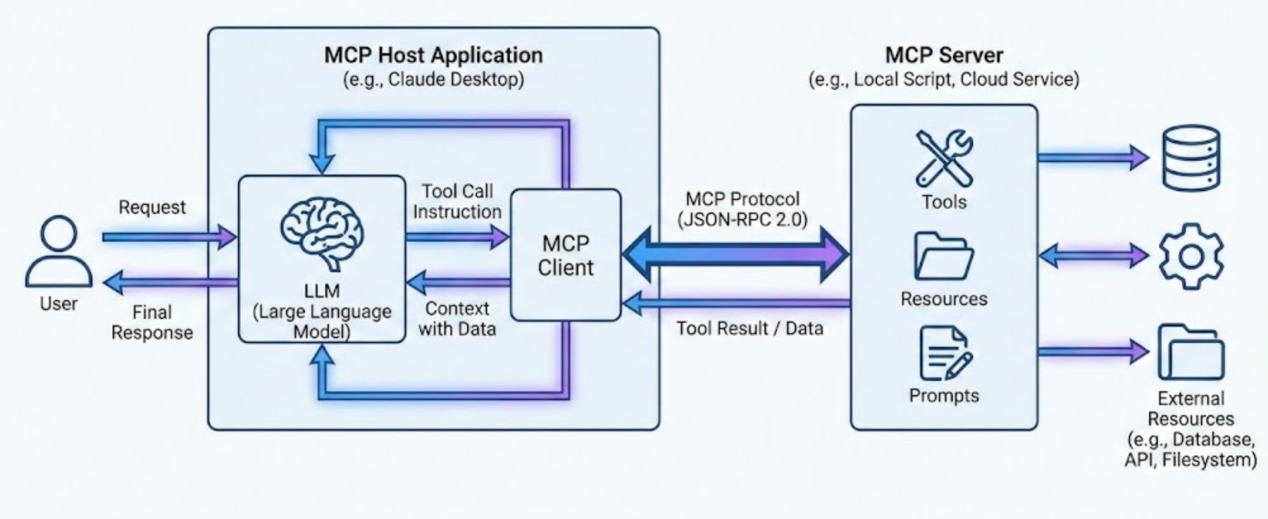
\includegraphics{images/image-0036.png}
\caption{围绕 KV Cache 设计上下文}
\end{figure}

\hypertarget{ux4e8cux5de5ux5177ux7ba1ux7406}{%
\subsection{二、工具管理}\label{ux4e8cux5de5ux5177ux7ba1ux7406}}

随着Agent能力的增强，其行动空间自然变得更加复杂，即工具数量爆炸式增长。如果允许用户自定义工具，总会有人将数百个神秘工具插入到行动空间中。结果，模型更可能选择错误的行动或采取低效的路径，Agent变得更加愚蠢。

一个自然的反应是设计一个动态行动空间，使用类似于RAG的方法按需加载工具，上下文中只包含这些被加载的工具。但实验表明，除非绝对必要，避免在迭代过程中动态添加或移除工具。这一方面是因为工具定义在上下文的前部，任何更改都会使后续所有动作和观察的KV缓存失效，另一方面是因为当先前的动作和观察仍然引用当前上下文中不再定义的工具时，模型会感到困惑，如果没有约束解码，这通常会导致模式违规或幻觉动作。

为了解决这个问题并仍然改进动作选择，有以下方法：

\begin{enumerate}
\def\labelenumi{\arabic{enumi}.}
\tightlist
\item
  只在上下文保留``元工具''，调用这些元工具会将模型导引到文件系统中具体工具存储的位置。这种设计本质上也是渐进式披露，好处在于让工具灵活且可扩展。
\end{enumerate}

以Claude Code的skills为例，\href{https://simonwillison.net/2025/Oct/16/claude-skills/\#skills-depend-on-a-coding-environment}{技能存储在文件系统}中，而非绑定工具，Claude只需调用几个简单的函数（如Bash、文件系统）即可逐步发现和使用技能，然后让模型自主提取需要的技能使用。这个过程只涉及会话上下文的累积，而不涉及上下文最前面工具定义的变化。

Manus也是如此，它只保留了不到20个``原子函数（Atomic Functions）''，如执行Bash命令、读写文件、执行Python代码。复杂的业务逻辑被包装成了沙盒里的CLI（命令行程序），模型不需要知道这几百个MCP工具的JSON Schema。模型只需要知道``我会用Bash''。当它需要使用MCP工具时，它直接在Bash工具里输入类似mcp-cli run some\_tool的命令即可。这里也不需要通过语义相似度的向量索引进行检索。

\begin{enumerate}
\def\labelenumi{\arabic{enumi}.}
\setcounter{enumi}{1}
\item
  只保留工具列表，让模型在需要的时候在文件系统中检索工具定义。GPT-5.4采取的就是这种策略。
\item
  在需要移除工具时，不直接将工具移出上下文，而是在解码过程中掩蔽token的logits，以基于当前上下文阻止（或强制）选择某些动作，或者通过prompt要求模型禁止使用特定工具（但这本质上变成了注意力机制的博弈，模型仍然有概率``违规操作''生成被禁用的工具）。
\end{enumerate}

\begin{figure}[htbp]
\centering
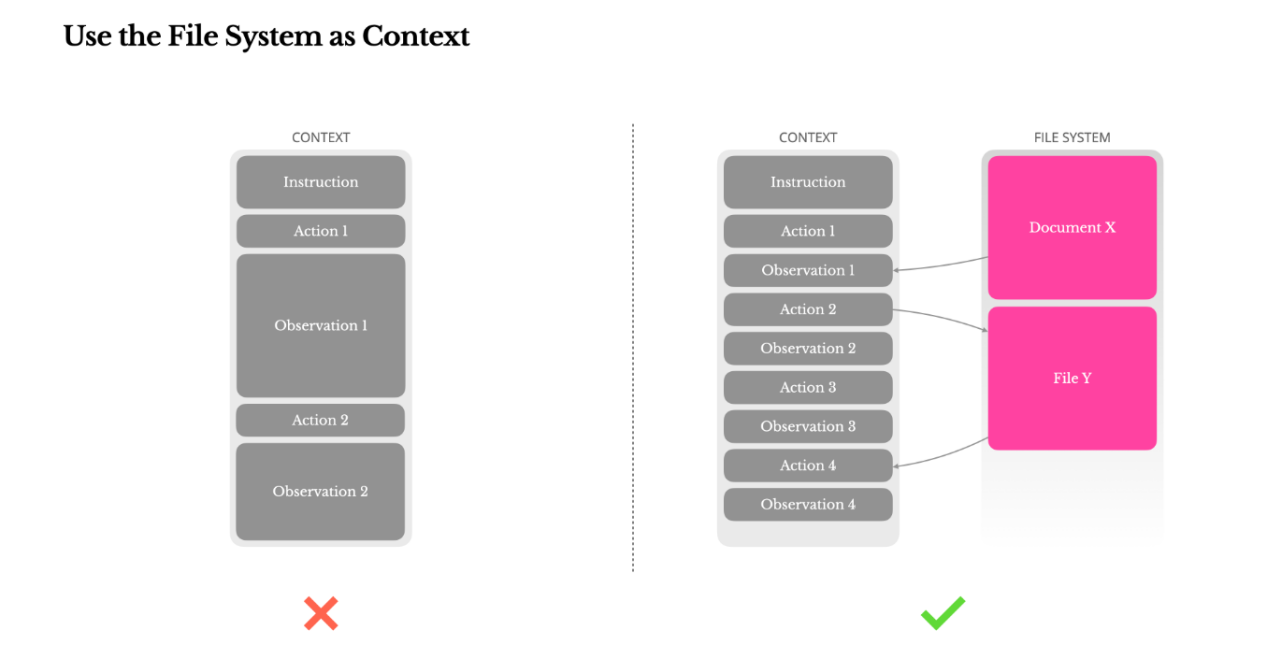
\includegraphics{images/image-0037.png}
\caption{通过掩蔽而非移除来管理工具}
\end{figure}

函数调用通常有三种模式：

自动：模型可以选择调用或不调用函数。通过仅预填充回复前缀实现：\textless\textbar im\_start\textbar\textgreater assistant

必需：模型必须调用函数，但选择不受约束。通过预填充到工具调用令牌实现：\textless\textbar im\_start\textbar\textgreater assistant\textless tool\_call\textgreater{}

指定：模型必须从特定子集中调用函数。通过预填充到函数名称的开头实现：\textless\textbar im\_start\textbar\textgreater assistant\textless tool\_call\textgreater\{``name'': ``browser\_''\}

\hypertarget{ux4e09ux4e0aux4e0bux6587ux7a97ux53e3-ux6587ux4ef6ux7cfbux7edfux5206ux5c42ux7ed3ux6784}{%
\subsection{三、``上下文窗口-文件系统''分层结构}\label{ux4e09ux4e0aux4e0bux6587ux7a97ux53e3-ux6587ux4ef6ux7cfbux7edfux5206ux5c42ux7ed3ux6784}}

上下文窗口有限，而信息的压缩是不可逆的。为此，我们可以只将重要信息留存在上下文窗口，其余则存储在文件系统中。模型学会按需写入和读取文件，不仅将文件系统用作存储，还用作结构化的外部记忆。

\begin{figure}[htbp]
\centering
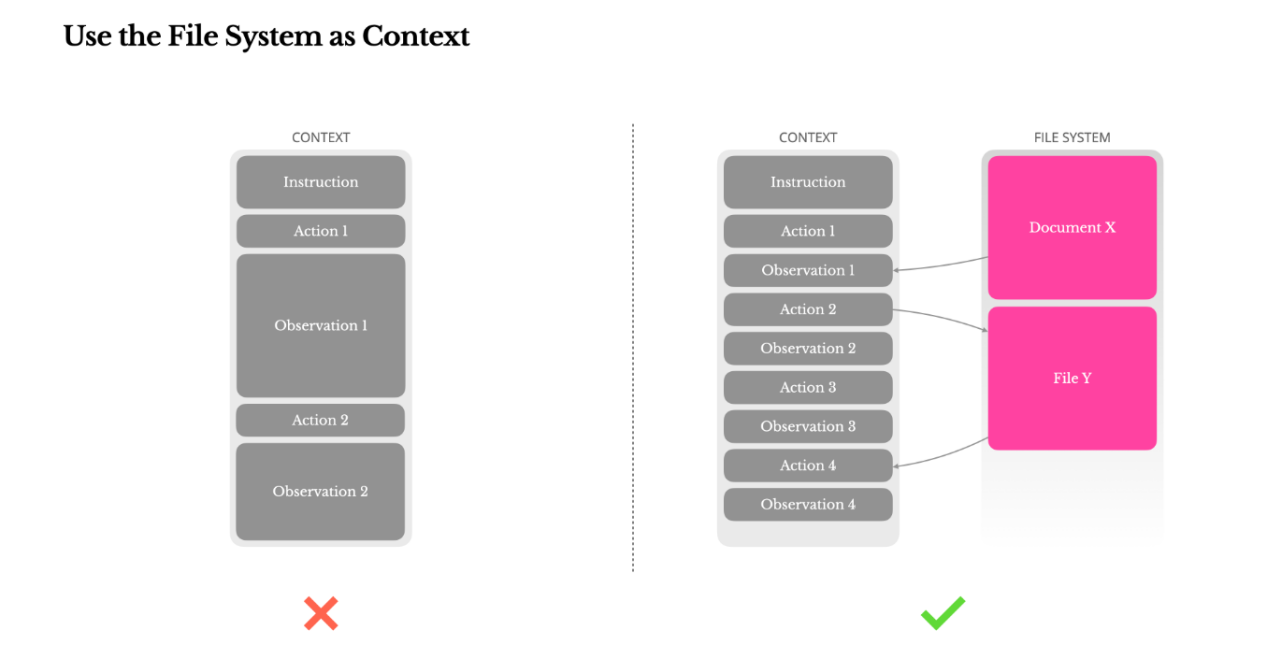
\includegraphics{images/image-0038.png}
\caption{将文件系统作为上下文}
\end{figure}

当上下文将满时，模型触发压缩（即在上下文最后加一条消息表示需要压缩）。对于工具调用结果，除了本轮会话以外，前面各轮会话的工具调用结果都会被压缩为指向文件系统中对应内容的索引。

\begin{figure}[htbp]
\centering
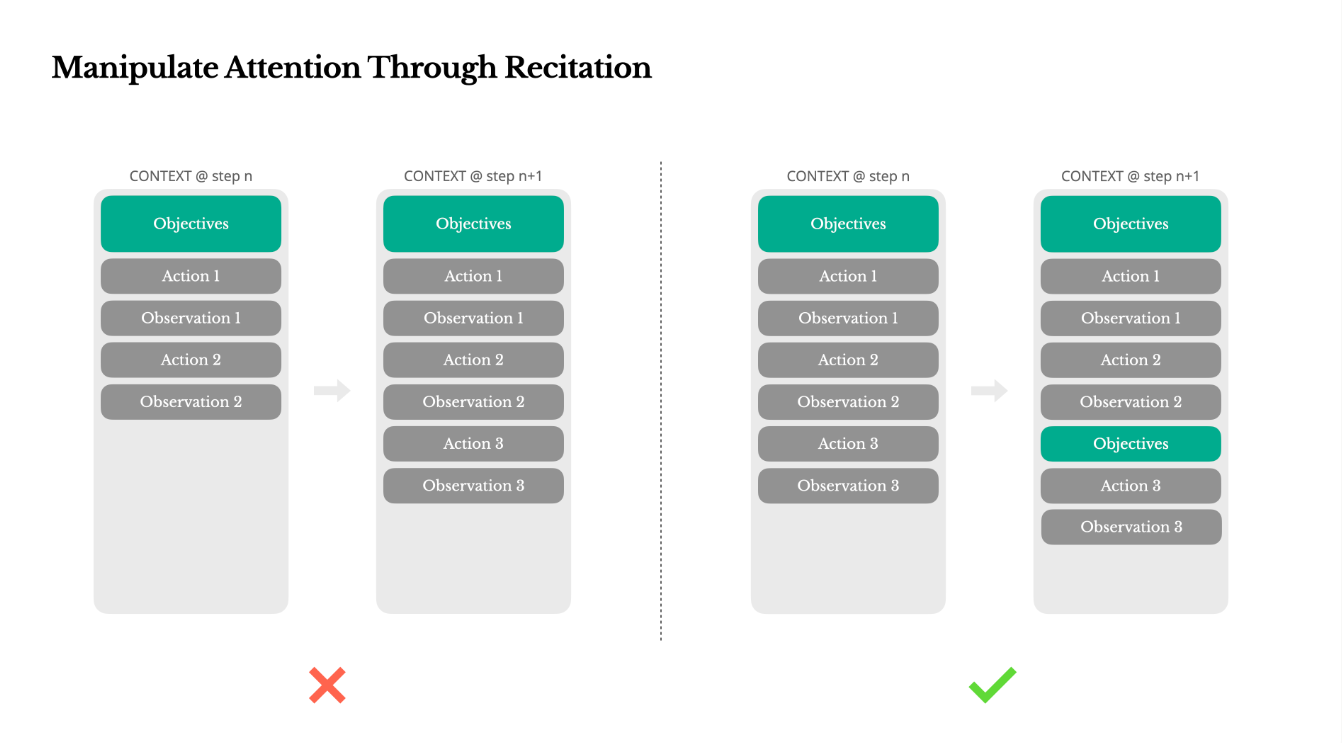
\includegraphics{images/image-0039.png}
\caption{压缩工具调用结果并保留必要内容}
\end{figure}

\hypertarget{ux56dbux590dux8ff0ux76eeux6807}{%
\subsection{四、复述目标}\label{ux56dbux590dux8ff0ux76eeux6807}}

在处理复杂任务时，很多Agent会倾向于创建类似于todo.md的计划文件，并在任务进行过程中逐步更新它，勾选已完成的项目。这不仅是为了方便用户审阅，更重要的是，这是在操控注意力，通过将其目标复述到上下文的末尾的方式，避免模型在复杂任务后期偏离目标。

\begin{figure}[htbp]
\centering
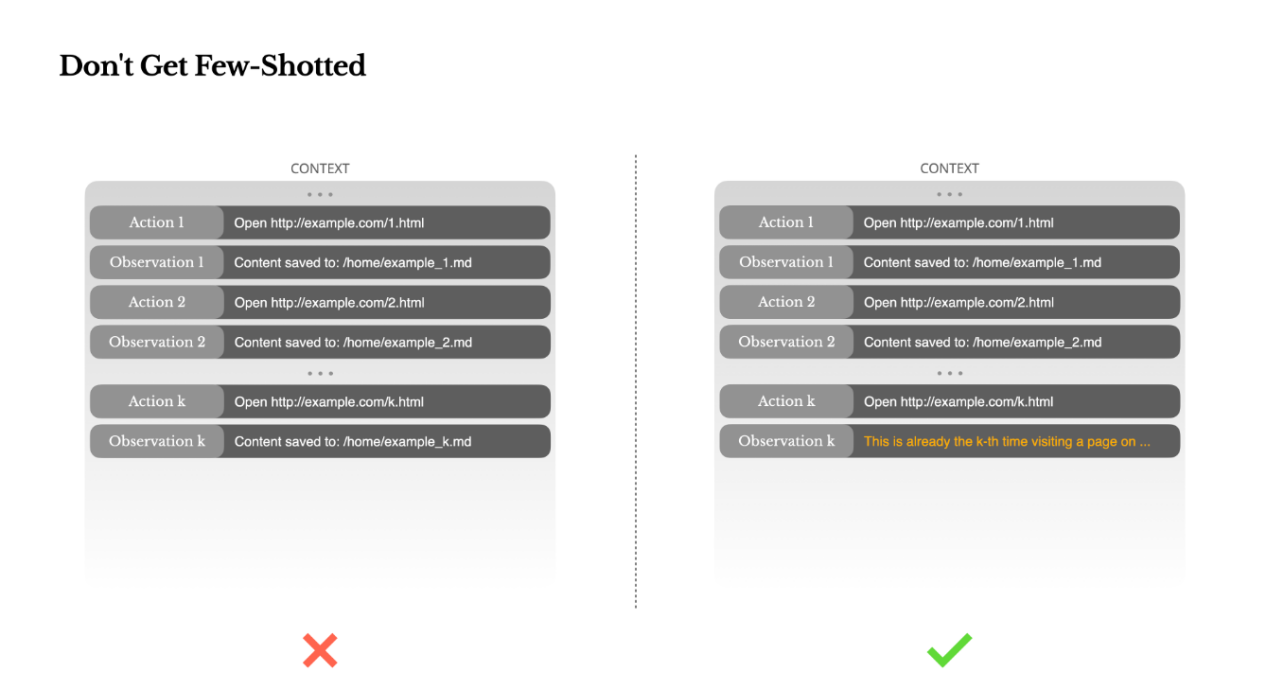
\includegraphics{images/image-0040.png}
\caption{通过复述目标操控注意力}
\end{figure}

\hypertarget{ux4e94ux4e0dux8981ux88abux5c11ux6837ux672cux793aux4f8bux6240ux56f0}{%
\subsection{五、不要被少样本示例所困}\label{ux4e94ux4e0dux8981ux88abux5c11ux6837ux672cux793aux4f8bux6240ux56f0}}

语言模型是优秀的模仿者；它们模仿上下文中的行为模式。如果上下文充满了类似的过去行动-观察对，模型将倾向于遵循该模式，即使这不再是最优的。这在涉及重复决策或行动的任务中可能很危险。例如，当审查20份简历时，代理通常会陷入一种节奏，即仅仅因为这是它在上下文中看到的，就重复与之类似的行动。这导致偏离、过度泛化，或有时产生幻觉。

解决方法是增加多样性，在行动和观察中引入少量的结构化变化，如不同的序列化模板、替代性措辞、顺序或格式上的微小噪音。这种受控的随机性有助于打破模式并调整模型的注意力。

\begin{figure}[htbp]
\centering
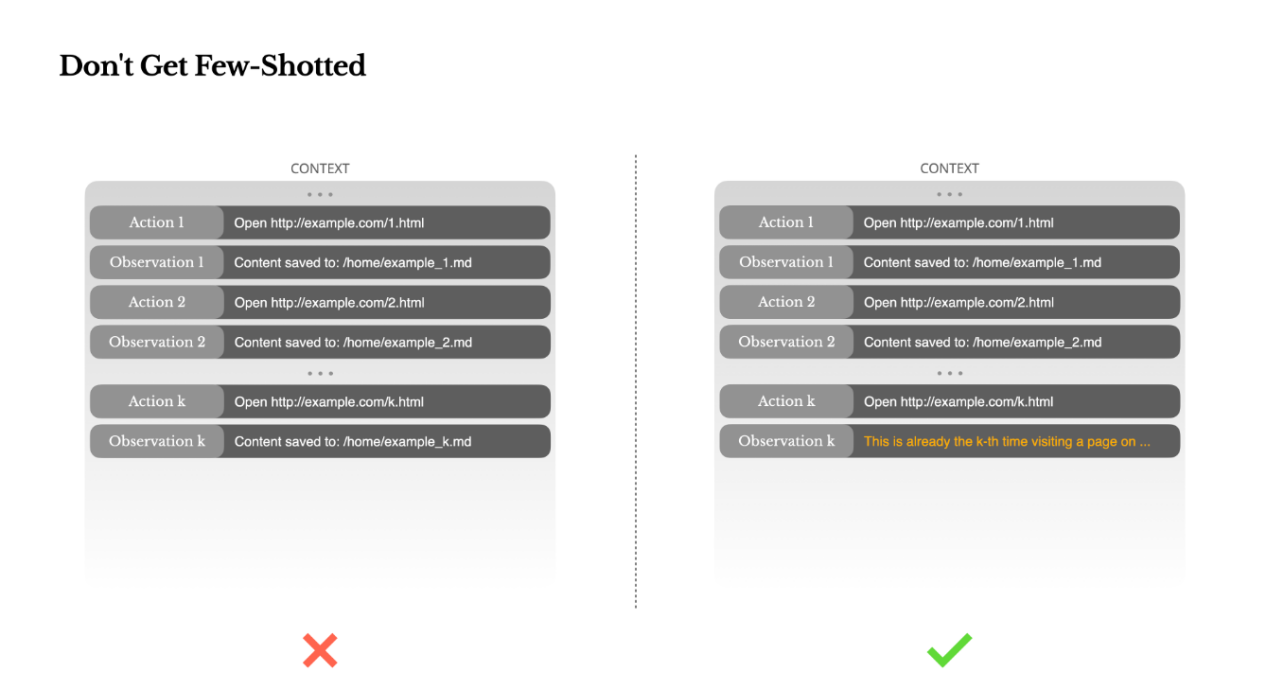
\includegraphics{images/image-0041.png}
\caption{避免少样本示例锁定行为模式}
\end{figure}

\hypertarget{ux516dux591aux667aux80fdux4f53ux7684ux4e0aux4e0bux6587ux9694ux79bb}{%
\subsection{六、多智能体的上下文隔离}\label{ux516dux591aux667aux80fdux4f53ux7684ux4e0aux4e0bux6587ux9694ux79bb}}

在多智能体系统中，主Agent和子Agent（如分别作为规划器和执行器）的上下文会存在一定隔离，如二者的system prompt和tools定义不同的。其余上下文可以不共享，但长上下文的复杂任务中仍建议共享。

不共享的范式：

\begin{figure}[htbp]
\centering
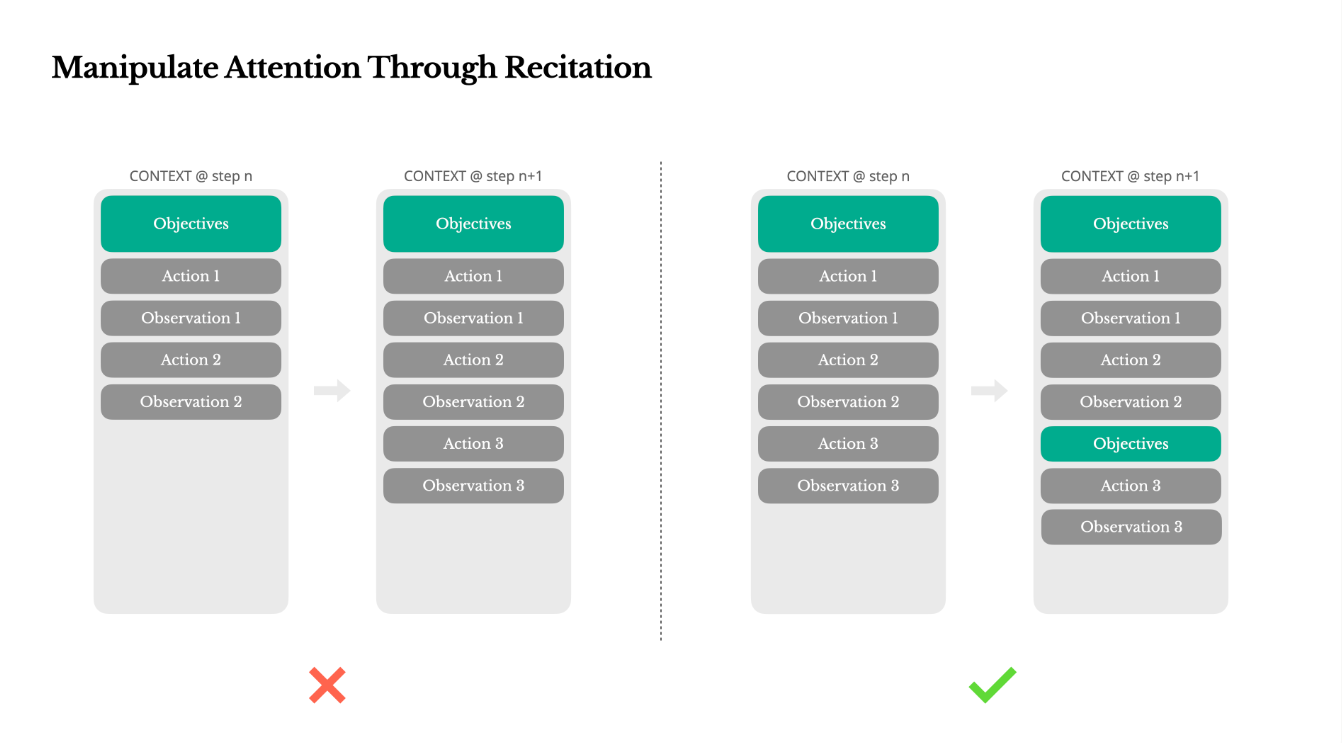
\includegraphics{images/image-0042.png}
\caption{主 Agent 与子 Agent 通过通信隔离上下文}
\end{figure}

部分共享的范式：（如主Agent作为规划者，与子Agent共享完整的上下文，子Agent仍拥有自己的动作空间（工具）和指令，但会获得规划者同样可访问的完整上下文。）

\begin{figure}[htbp]
\centering
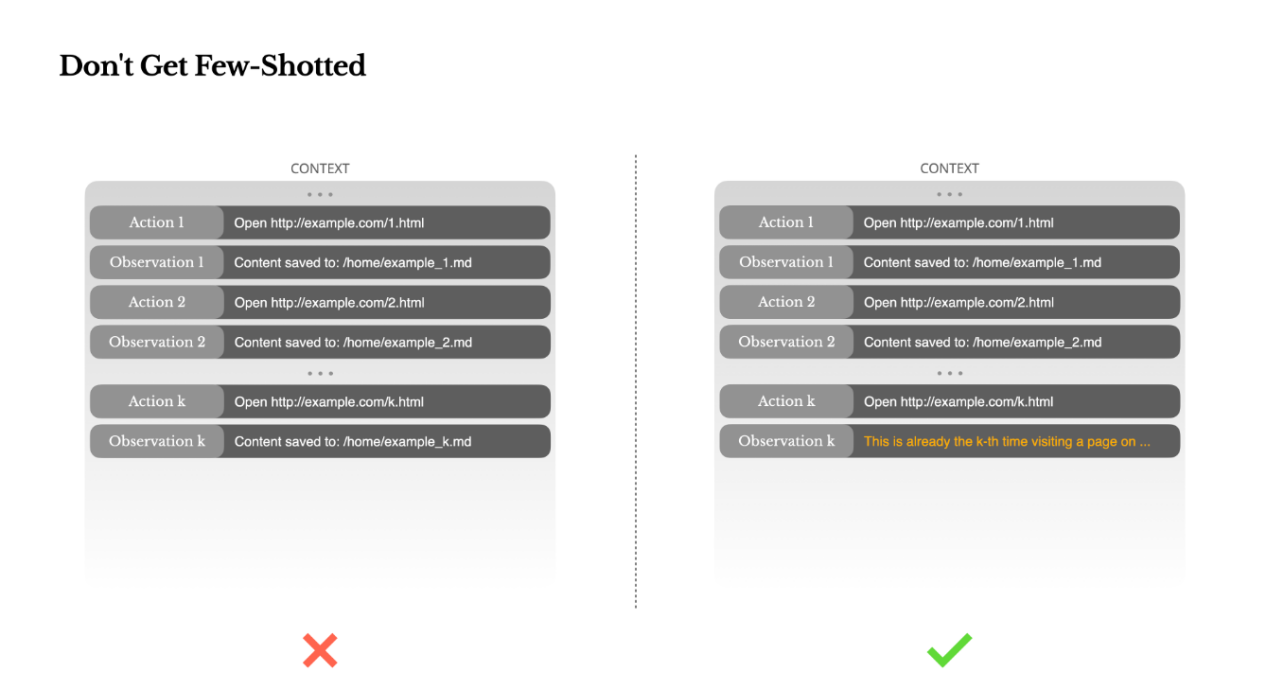
\includegraphics{images/image-0043.png}
\caption{主 Agent 与子 Agent 共享上下文}
\end{figure}

\hypertarget{ux53c2ux8003ux6587ux732e-126}{%
\subsection{参考文献}\label{ux53c2ux8003ux6587ux732e-126}}

\vspace{0.25em}
\begin{itemize}
\tightlist
\item
  Martin, L. (2025). \href{https://rlancemartin.github.io/2025/10/15/manus/}{Context Engineering for Agents}.
\item
  Manus. (2025). \href{https://manus.im/zh-cn/blog/Context-Engineering-for-AI-Agents-Lessons-from-Building-Manus}{Context Engineering for AI Agents: Lessons from Building Manus}.
\end{itemize}

\clearpage
